\section{Векторизация}

\subsection{Простая векторизация}

\begin{frame}{Глобальные статистики}

Какая глобальная информация о картинке может быть полезна для её поиска?

\begin{itemize}
    \item Гистограмма всех цветов (яркости).
    \item Переход в другое цветовое представление и гистограмма в нём.
    \item Применить преобразование Фурье, и смотреть статистики частот.
    \item Выбрать набор текстур, и описывать картинки через наличие в них таких текстур.
\end{itemize}

А ещё...

\pause
\begin{itemize}
    \item Представить картинку как взвешенную сумму других картинок.
\end{itemize}
    
\end{frame}

\begin{frame}{Разложение на базис}

Можно использовать кластеризацию для нахождения <<средних>> изображений, из которых будут составляться остальные.

\centering
\begin{tabular}{cc}
    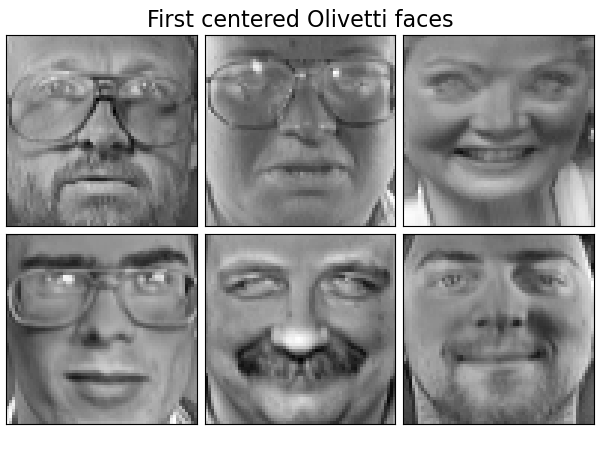
\includegraphics[width=0.4\textwidth]{images/faces/sphx_glr_plot_faces_decomposition_001.png} &
    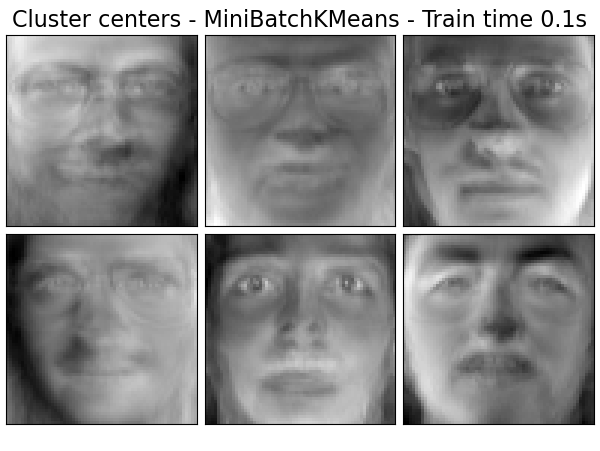
\includegraphics[width=0.4\textwidth]{images/faces/sphx_glr_plot_faces_decomposition_007.png}
\end{tabular}

\alternativefootnote{\url{https://scikit-learn.org/stable/auto_examples/decomposition/plot_faces_decomposition.html}}
\end{frame}

\begin{frame}{Разложение на базис}

Можно вспомнить  метод главных компонент, чтобы найти нужный базис.

\centering
\begin{tabular}{cc}
    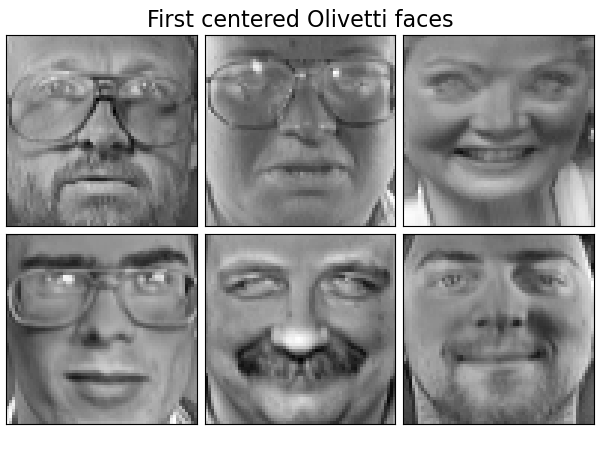
\includegraphics[width=0.4\textwidth]{images/faces/sphx_glr_plot_faces_decomposition_001.png} &
    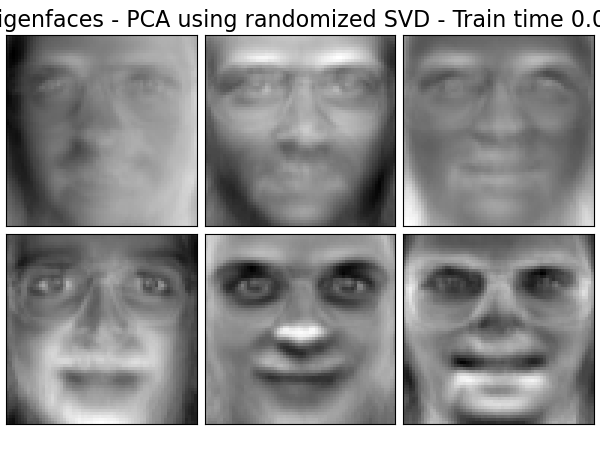
\includegraphics[width=0.4\textwidth]{images/faces/sphx_glr_plot_faces_decomposition_002.png}
\end{tabular}

\alternativefootnote{\url{https://scikit-learn.org/stable/auto_examples/decomposition/plot_faces_decomposition.html}}
\end{frame}

\begin{frame}{Разложение на базис}

Или даже добавить ограничение неотрицательности, чтобы полученные матрицы можно было хоть как-то считать картинками.

\centering
\begin{tabular}{cc}
    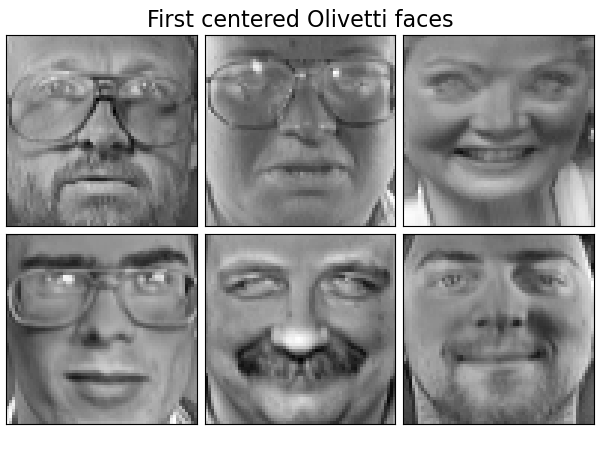
\includegraphics[width=0.4\textwidth]{images/faces/sphx_glr_plot_faces_decomposition_001.png} &
    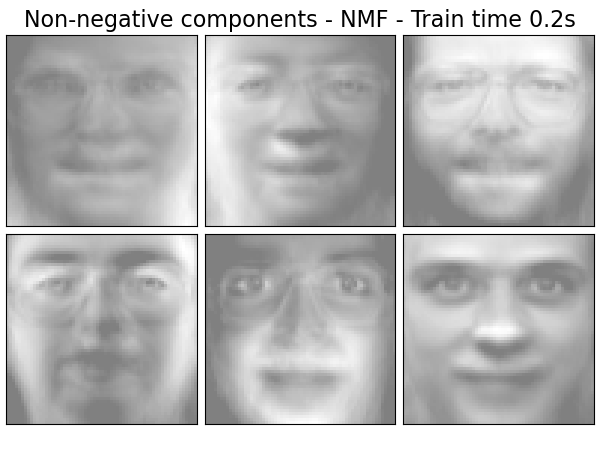
\includegraphics[width=0.4\textwidth]{images/faces/sphx_glr_plot_faces_decomposition_003.png}
\end{tabular}

\alternativefootnote{\url{https://scikit-learn.org/stable/auto_examples/decomposition/plot_faces_decomposition.html}}
\end{frame}

\subsection{CNN как векторизатор}

\begin{frame}{Дескрипторы классификационной CNN}

\begin{itemize}
    \item Свёрточные нейросети умеют правильно классифицировать картинки.
    \item Внутреннюю информацию можно извлечь и использовать в качестве описания картинки!
\end{itemize}

\centering
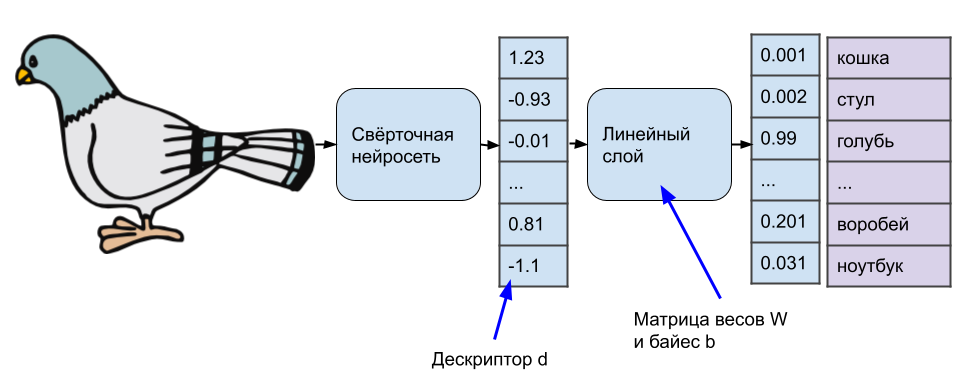
\includegraphics[width=0.8\textwidth]{images/pigeon CNN.png}

Итоговые предсказания класса $i$: $ \sigma_i(W^\Tr_i d + b_i) = \frac{\exp ( W^\Tr_i d + b_i )}{\sum_j \exp ( W^\Tr_j d + b_j )}$
    
\end{frame}

\begin{frame}{Вспоминаем задачу классификации}

Мы пытаемся минимизировать кроссэнтропию:
\[
CE(X,\,Y) = - \frac{1}{B} \sum_{k=1}^{B} \ln \frac{e^{W_{y_k}^\Tr d_k + b_{y_k}}}{ \sum_{j=1}^{N} e^{ W_{j}^\Tr d_k + b_{j} } } \rightarrow \min_{W,\,b,\,d}
\]

Сконцентрируемся только на одном объекте класса $i$:

\[
- \ln \frac{e^{W_{i}^\Tr d + b_i}}{ \sum_{j=1}^{N} e^{ W_{j}^\Tr d + b_{j} } } = 
\ln \left( \sum_{j=1}^{N} e^{ W_{j}^\Tr d + b_{j} } \right) - \ln e^{W_{i}^\Tr d + b_i} = 
\ln \left( \sum_{j=1}^{N} e^{ W_{j}^\Tr d + b_{j} } \right) - \left( W_{i}^\Tr d + b_i \right)
\]

Мы хотим, чтобы дескриптор $d$ был похож на столбец $W_i$ больше, чем на другие столбцы!
    
\end{frame}


\subsection{Angular Loss}

\begin{frame}{Минимизация угла}

Ещё раз про классификацию из дескриптора:
\[
\sigma_i(W^\Tr_i d + b_i) = \frac{\exp ( W^\Tr_i d + b_i )}{\sum_j \exp ( W^\Tr_j d + b_j )}
\]

Если мы отнормируем дескиптор $d$ и столбцы $W$, то скалярное произведение внутри экспоненты можно переписать:

\[
\frac{\exp ( \|W_i\|_2 \|d\|_2 \cos \theta_{i} + b_i )}{\sum_j \exp ( \|W_j\|_2 \|d\|_2 \cos \theta_{j} + b_j )} = \{ \|d\|_2 = 1,\, \|W_i\|_2 = 1 \} = 
\frac{\exp ( \cos \theta_{i} + b_i )}{\sum_j \exp ( \cos \theta_{j} + b_j )}
\]

В этом случае мы уменьшаем непосредственно угол между дескриптором и нужным столбцом матрицы $W$.
    
\end{frame}

\begin{frame}{Angular Loss}

А что если нам идею с зазором добавить в оптимизируемый нами угол?
\[
AngularLoss : \frac{e^{ \cos (m_1 \theta_{i} + m_2) + m_3} }{e^{ \cos (m_1 \theta_{i} + m_2) + m_3} + \sum_{j \neq i} e^{ \cos \theta_{j}} }
\]

\centering
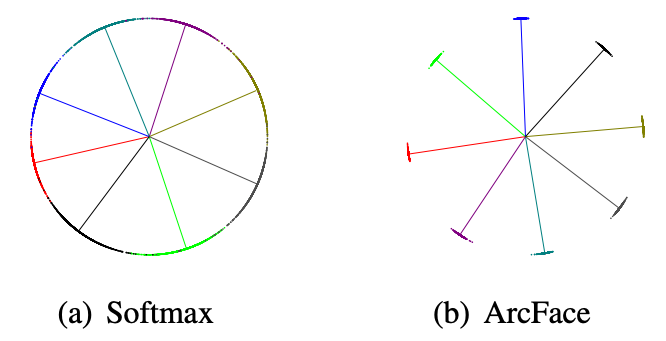
\includegraphics[width=0.5\textwidth]{images/arcface.png}
    
\end{frame}


\subsection{Обучение метрики}

\begin{frame}{Сиамские сети, обучения по парам}
\centering
\begin{tabular}{m{15em} m{10em}}
    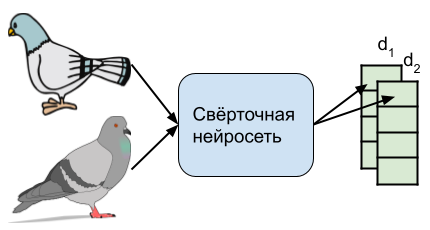
\includegraphics[width=0.38\textwidth]{images/siamse pigeon1.png} & 
    $
    \min_{d_1,\,d_2} \left( 1 - \frac{ d_1^\Tr d_2 }{\|d_1\|_2 \|d_2\|_2} \right)
    $
    \\
    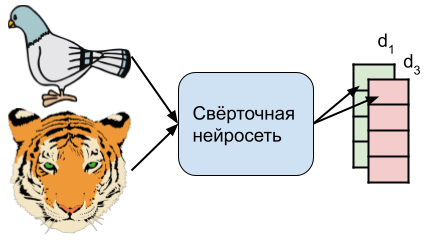
\includegraphics[width=0.38\textwidth]{images/siamse pigeon2.png} & 
    $
    \max_{d_1,\,d_3} \left( 1 - \frac{ d_1^\Tr d_3 }{\|d_1\|_2 \|d_3\|_2} \right)
    $
    \\
\end{tabular}

Если передавать метку $1$ для положительных пар и $-1$ для отрицательных, функцию ошибки можно записать в общем виде: $y_{ij} \left( 1 - \frac{ d_i^\Tr d_j }{\|d_i\|_2 \|d_j\|_2} \right) \rightarrow \min_{d_1,\,d_2}$

\end{frame}

\begin{frame}{Триплеты, схемы семплирования}

\begin{tabular}{m{14em} m{15em}}
    
\includegraphics[width=0.4\textwidth]{images/pigeon triplet1.png} &  
    --- случайное семплирование \\
    
\includegraphics[width=0.4\textwidth]{images/pigeon triplet2.png} &  
    --- semi-hard negative sampling \\
    
\includegraphics[width=0.4\textwidth]{images/pigeon triplet3.png} &  
    --- hard negative sampling, hard positive sampling
\end{tabular}

Мы хотим, чтобы расстояние от якорного примера до положительного было меньше, чем до отрицательного.

Hinge loss: $ [ m + dist(d_A, d_P) - dist(d_A, d_N) ]_+ $
    
\end{frame}

\begin{frame}{Ещё обучения метрики}

\begin{itemize}
    \item Можно добавить пару к негативному примеру, получим квадруплеты!
    \item Можно пользоваться особенностью обучения по батчам, и семплировать примеры только изнутри батча.
    \item Используя матричные формы функции ошибки можно без семплирования оптимизировать сразу по всем возможным парам из батча.
    \item Можно формировывать псевдо-классы. И вместо отсемплированных примеров, брать эти псевдоклассы (Proxy-NCA).
    \item И ещё много идей...
\end{itemize}
    
\end{frame}

\begin{frame}{Но в реальности...}

Так всё это обучение метрик вообще помогает?

\begin{center}
    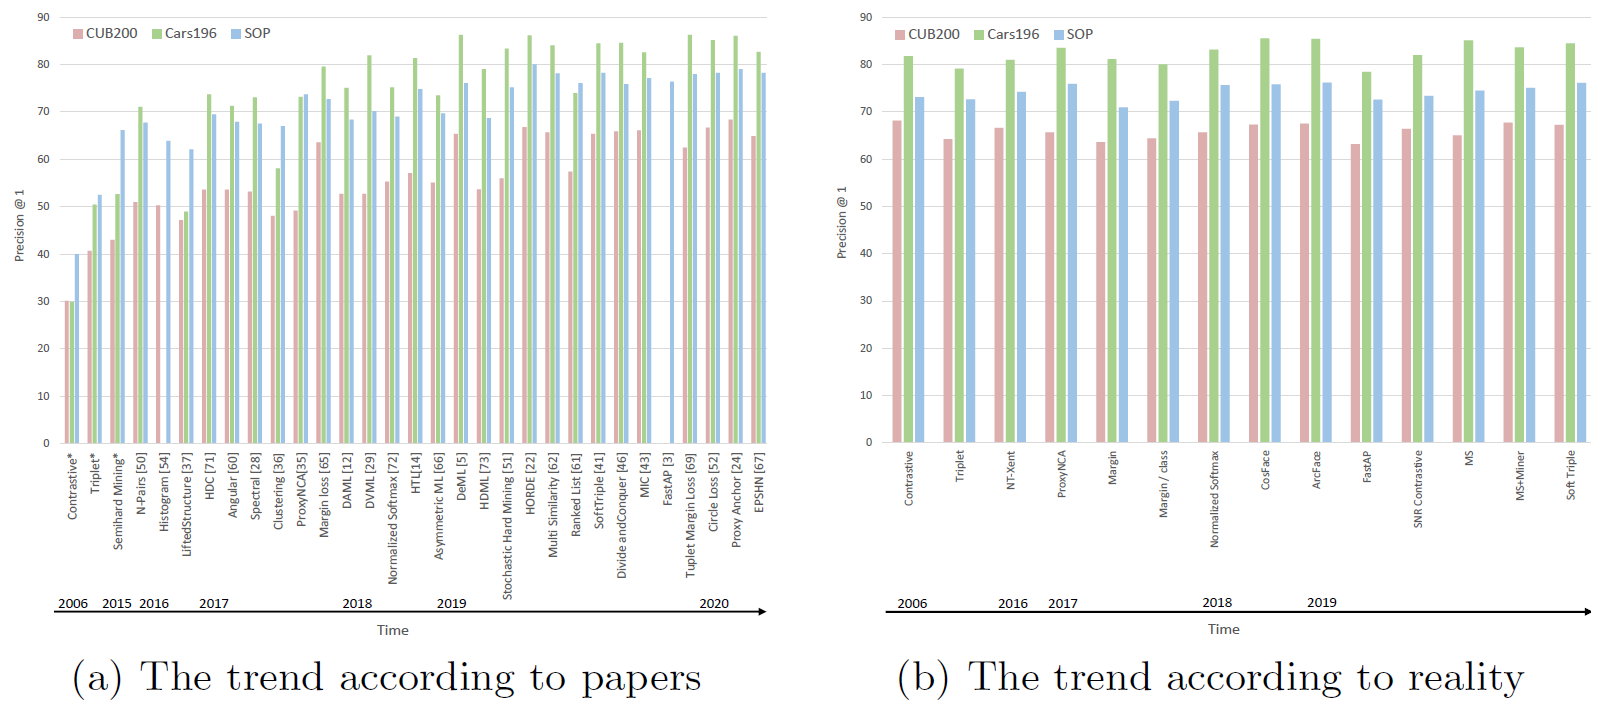
\includegraphics[width=0.9\textwidth]{images/reality check.png}
\end{center}

\alternativefootnote{\fullcite{musgrave2020metric}}
\end{frame}

